\documentclass[12pt]{article}
\usepackage{graphicx}
\usepackage{amsmath}
\usepackage[utf8]{inputenc}
\usepackage{titlesec}
\setcounter{secnumdepth}{4}
\usepackage{sectsty}
\usepackage[utf8]{inputenc}
\usepackage[T1]{fontenc}
\usepackage{hyperref}
\hypersetup{
    colorlinks=true, 
    linktoc=none, 
    linkcolor=blue,
}
\usepackage[a4paper, total={6in, 8in}]{geometry}
\renewcommand*\contentsname{Table of Contents}

\begin{document}

\begin{titlepage}
    \begin{center}
        \vspace*{1cm}
        
        \Large
        \textbf{Introduction to Robotics (UE15EE347)}
        
        \vspace{0.5cm}
        \LARGE
        Mini Project
        \vspace{0.5cm}
        
MOPBOT\\
Smart and autonomous mopping of floors\\
\vspace{0.5cm}
By\\
Kenneth Joel (01FB15EEE015)\\
Mohan S P (01FB15EEE019)\\

        \vspace{0.8cm}
Guided by: Prof. Venkatrangan M.J
        
        
\includegraphics[width=0.4\textwidth]{university.jpg}
        
        \Large
        Department of Electrical and Electronics Engineering\\
        PES University\\
        Bengaluru-560085\\
    \end{center}
\end{titlepage}
 
\tableofcontents

\newpage

\part{Literature review}

\section{Objective}

To enable autonomous mopping of floors using a mobile robot equipped with sensors and necessary actuators

\begin{itemize}
\item Plan a path for the room such that the entire surface is optimally covered.
\item Mopping the floor by means of a robotic actuator.
\end{itemize}

\section{Introduction}

Robots for household cleaning purposes have seen widespread acceptance over the past few years. Taking inspiration from this we intend to design one of our own so we gain some exposure to the challenges associated with the development of such products.
We hope to develop a prototype of an autonomous house mopping bot taking inspiration from a few commercially available products.
  
\section{Methodology}

Interface the following components with Firebird V
\begin{itemize}
\item DC Motors (For movement of the bot)
\item LCD (For debugging)
\item Sharp IR sensor (To measure the distance from any obstacle while navigating) 
\item Ultrasound (To measure the distance from the wall while navigating)
\item Servo motors (To enable the motion of the actuator)
\end{itemize}

\noindent After interfacing all the above components successfully integrate all of them to make MOPBOT. 

\part{Hardware used}

\section{Firebird V by Nex Robotics}

\begin{center}
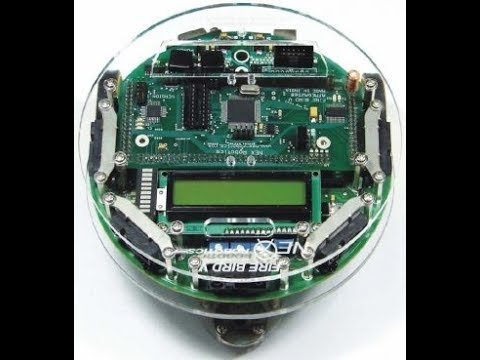
\includegraphics[width=0.3\textwidth]{1.jpg}
\end{center}

\section{MeArm}

\begin{center}
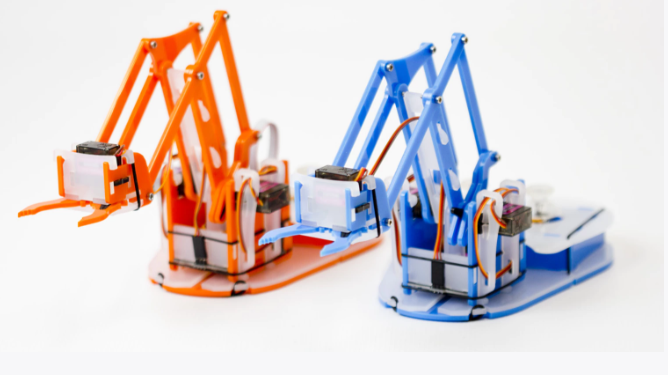
\includegraphics[width=0.3\textwidth]{2.jpg}
\end{center}

\section{Ultrasound sensor}

\begin{center}
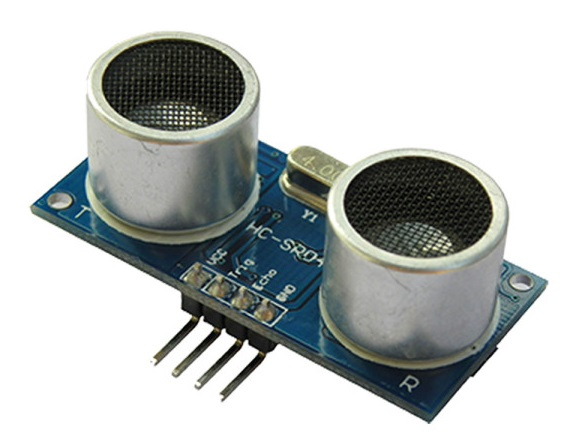
\includegraphics[width=0.2\textwidth]{3.jpg}
\end{center}

\section{Sharp IR sensor}

\begin{center}
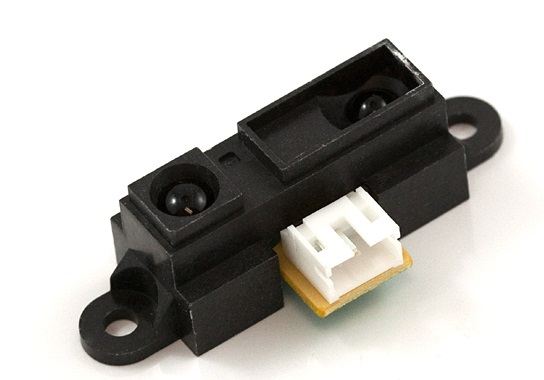
\includegraphics[width=0.2\textwidth]{4.jpg}
\end{center}

\part{Mathematical modeling of MeArm}

Given below is the DH representation of the MeArm.

\begin{center}
\begin{tabular}{ |p{0.9cm}|p{0.7cm}|p{0.9cm}|p{0.3cm}|}
\hline
 $a_{i-1}$ & $\alpha_{i-1}$ & $d_{i}$ & $\theta_{i}$ \\
\hline
$0.0 cm$ & $0^{\circ}$ & $3.0 cm$ & $\theta_{1}^{\circ}$ \\
\hline
$1.5 cm$ & $-90^{\circ}$ & $2.7 cm$ & $\theta_{2}^{\circ}$ \\
\hline
$8.5 cm$ & $0^{\circ}$ & $0.0 cm$ & $\theta_{3}^{\circ}$ \\
\hline
$8.0 cm$ & $0^{\circ}$ & $0.0 cm$ & $0^{\circ}$ \\
\hline
\end{tabular}
\end{center}

\noindent Using the above representation the transformation matrix from the universal frame to the end effector was obtained as shown below

\begin{center}
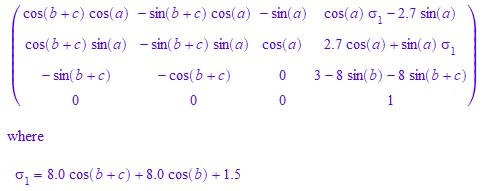
\includegraphics[width=0.5\textwidth]{5.jpg}
\end{center}

\part{Software architecture}

\begin{center}
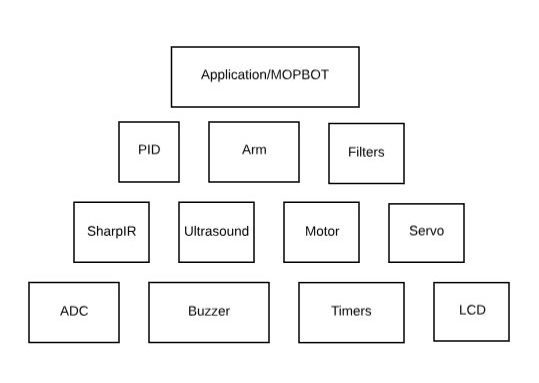
\includegraphics[width=0.5\textwidth]{6.jpg}
\end{center}

\part{Flowcharts}

\begin{center}
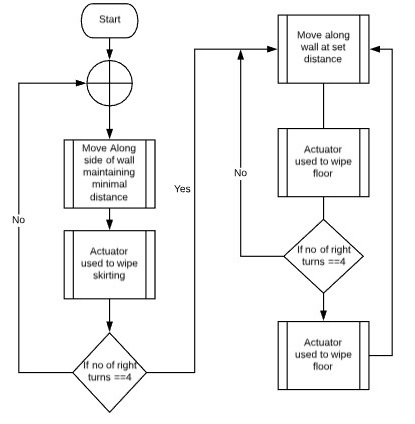
\includegraphics[width=0.5\textwidth]{7.jpg}
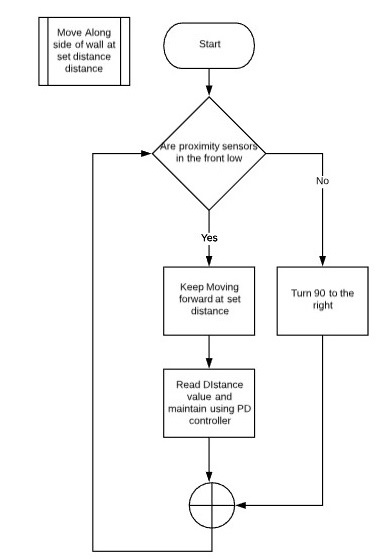
\includegraphics[width=0.5\textwidth]{8.jpg}
\end{center}

\part{Design details}

The design specifications of the project can be broadly classified into 

\begin{itemize}
\item Navigation
\item Actuator kinematics
\end{itemize}

\section{Navigation}
The core problem statement of the navigation aspect of this project was to efficiently cover the floor space to be cleaned. The approaches we took are described in the flowcharts that are shown later on in this report. However, one key design concern was obtaining reliable distance data from the left and front of the bot. To ensure quality of this data a few steps were taken. \\ \\
Firstly, a moving average of sensor data was taken to act as a low pass filter, the length of this filter depended on both the type of sensor and the type of response required. \\ \\
Secondly, it was found that due to the angle the bot makes while turning to correct itself as instructed by the controller there is sometimes an error in the sensor reading, to take care of this, two sensors of the same type are used on the left side and the lower of the two readings is considered as the true distance. This point is illustrated in the figure below.

\begin{center}
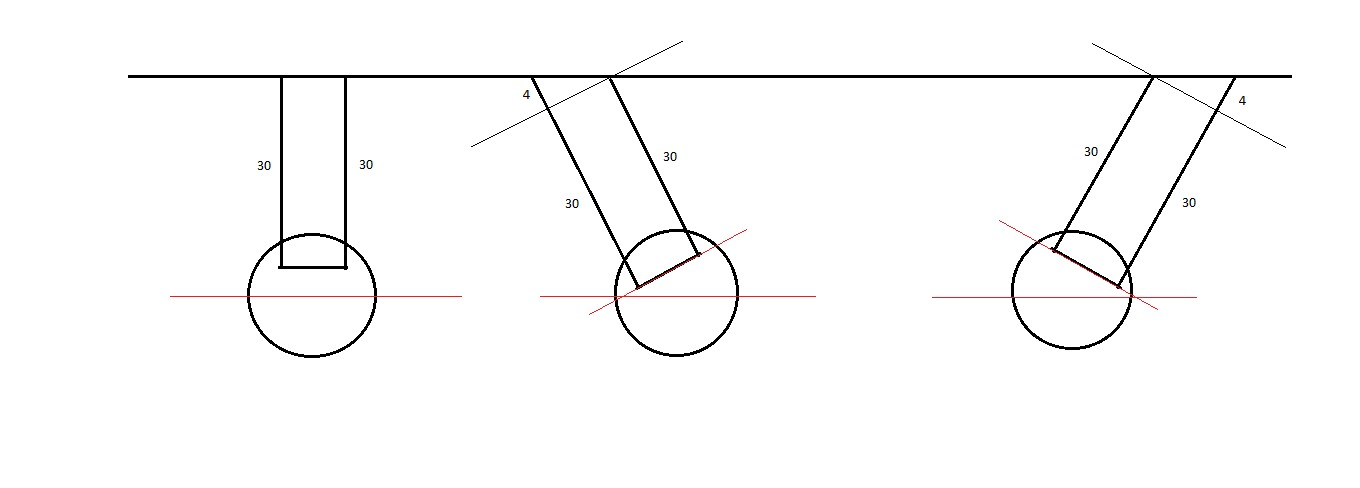
\includegraphics[width=0.9\textwidth]{9.jpg}
\end{center}
 
\noindent Lastly, the P controller used had a dead band that helped reduce the over-sensitivity of the system and helped it stay on a straight path. 

\subsection{Ultrasound sensor interfacing code}
The ultrasound sensor we used was a time-based distance measurement sensor. Since, we wanted to interface two ultrasound sensors and we were running short of timers we decided to use a single timer and operate the two ultrasounds serially. The code is as shown below\\

\paragraph{Timer initialization} 
\begin{center}
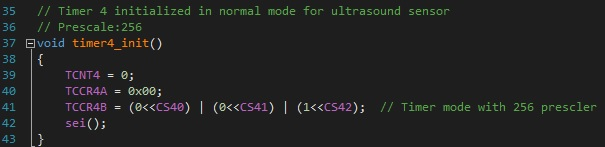
\includegraphics[width=0.9\textwidth]{10.jpg}
\end{center}

\paragraph{Port Initialization}
\begin{center}
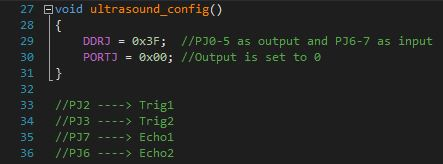
\includegraphics[width=0.9\textwidth]{11.jpg}
\end{center}

\paragraph{Trigger pin function}
\begin{center}
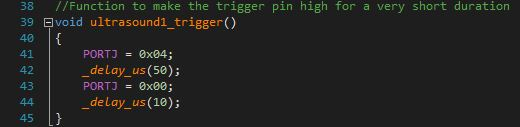
\includegraphics[width=0.9\textwidth]{12.jpg}
\end{center}

\newpage
  
\paragraph{Distance calculation}
\begin{center}
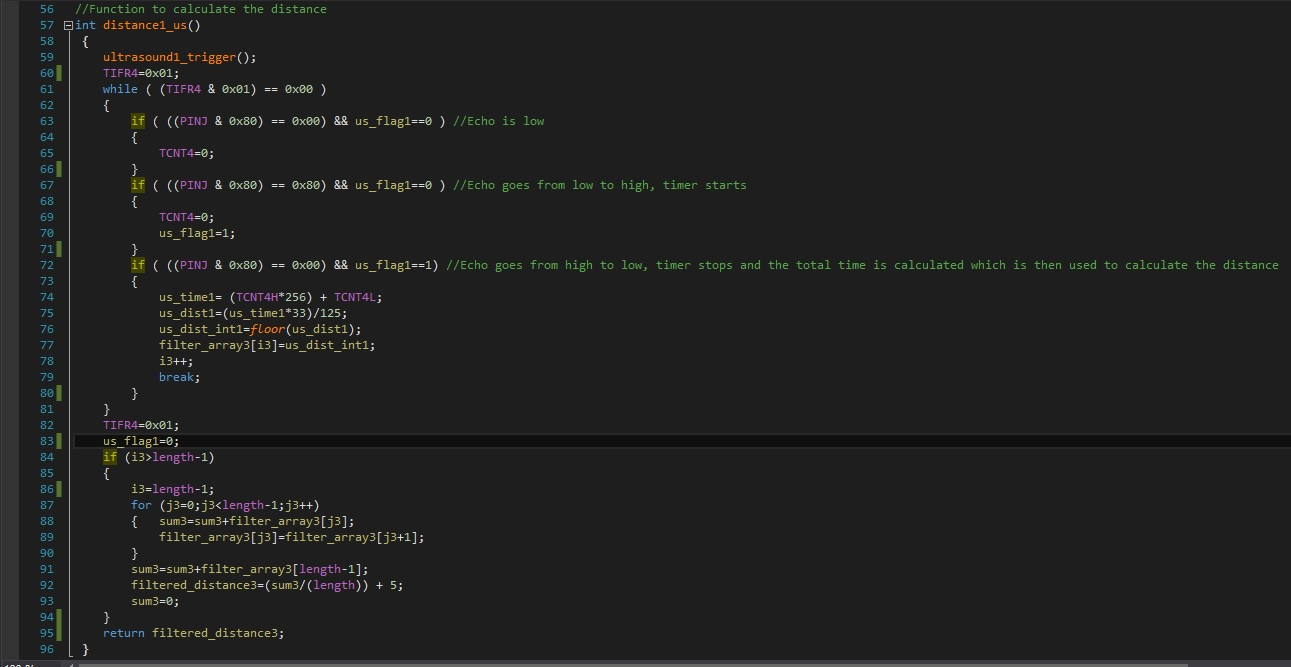
\includegraphics[width=1.0\textwidth]{13.jpg}
\end{center} 

\subsection{Sharp IR sensor interfacing code}
Unlike the ultrasound sensor, this gave a voltage based distance measurement. Therefore using ADC the voltage values were directly converted to distance using a relation given by the manufacturer.\\

\paragraph{Distance calculation}
\begin{center}
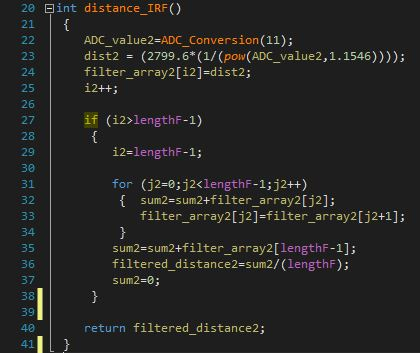
\includegraphics[width=0.5\textwidth]{14.jpg}
\end{center}

\newpage

\subsection{P control with deadband for navigation}
\begin{center}
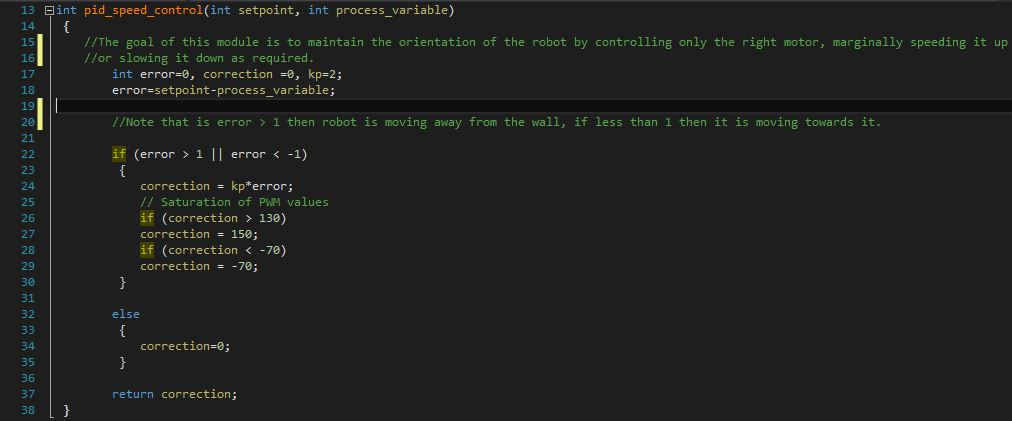
\includegraphics[width=0.8\textwidth]{15.jpg}
\end{center}

\section{Actuator kinematics}
Working with the servos at a relatively lower lever gave us a greater degree of control over the motor. The mathematical model of the arm was first derived by hand. These equations were then substituted in MuPad and then solved for, in MATLAB.\\ \\
Care was taken to ensure that solutions provided is out of the reachable workspace by using thresholds to limit angles. Once point solutions were found and verified using inverse kinematics solutions, linear trajectories were solved for to generate the cleaning motion.\\ \\
Power for the servo was not an issue as the Firebird V provides 3 ports that are dedicated for these high current applications.\\  

\subsection{Servo interface}

\paragraph{Timer initialization}
\begin{center}
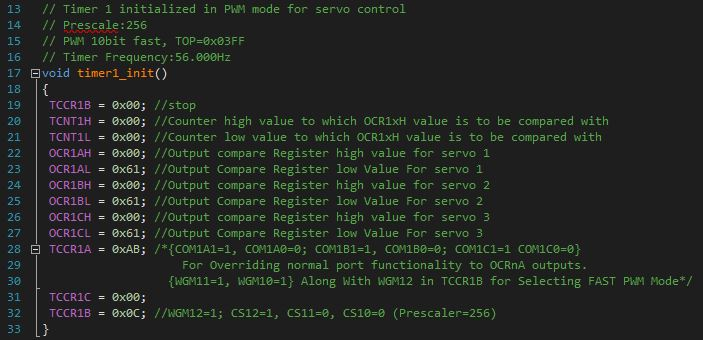
\includegraphics[width=0.5\textwidth]{16.jpg}
\end{center}

\paragraph{Port initialization}
\begin{center}
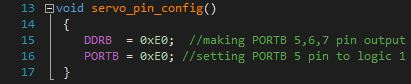
\includegraphics[width=0.7\textwidth]{17.jpg}
\end{center}

\paragraph{Degree calculation\\}
\noindent Servo uses the technique of PPM(Pulse Position Modulation) to turn to specified degrees. So first we took a few standard points such as $0^{\circ}$, $90^{\circ}$ and $180^{\circ}$. Once we got the timer values for these angles, we linear curve-fit the data in Microsoft Excel to obtain the relation between timer values and degrees moved by the servo as shown below.

\begin{center}
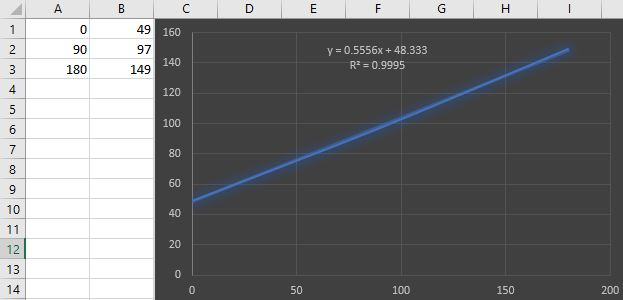
\includegraphics[width=0.7\textwidth]{18.jpg}
\end{center}

\noindent After obtaining the general relation as shown above we implemented the same in a function to turn the servo to any desired angle between $0^{\circ}$ and $180^{\circ}$ as shown below.

\begin{center}
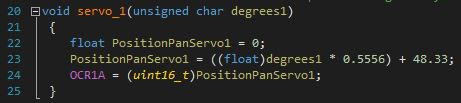
\includegraphics[width=0.7\textwidth]{19.jpg}
\end{center}

\noindent Using the above mathematical model and servo interface we obtained joint angles for the desired trajectories and coded it so that the actuator performs the desired cleaning actions.

\section{MATLAB implementation of MeArm}
\begin{center}
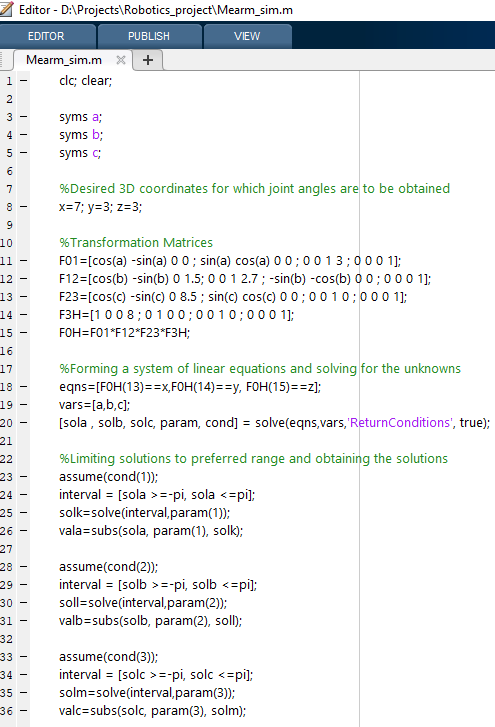
\includegraphics[width=0.8\textwidth]{20.jpg}
\end{center}

\newpage

\section{Navigation implementation}
Using all the above obtained results and our decided algorithm for navigation, the navigation part of the project is as shown below.

\begin{center}
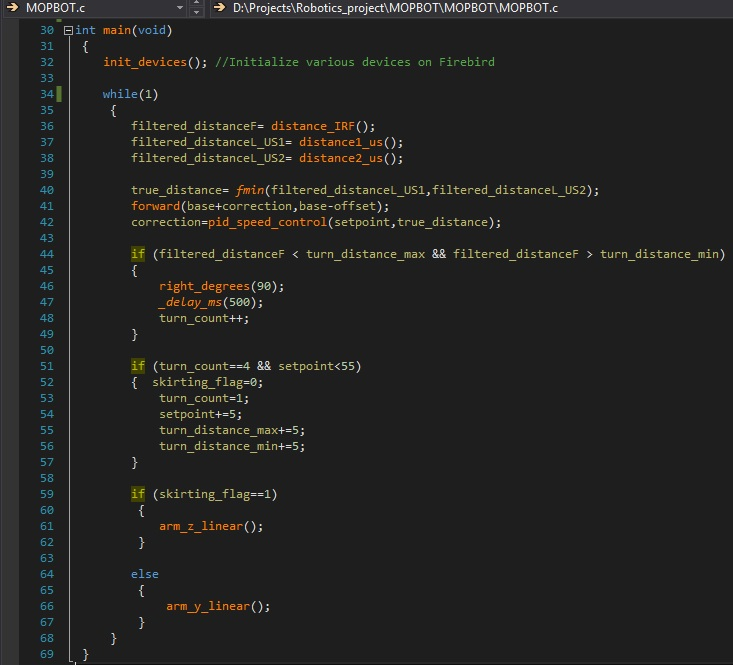
\includegraphics[width=1.1\textwidth]{21.jpg}
\end{center}

\part{Learning experience}

\section{Indoor navigation}

\begin{itemize}
\item Developing a module for the ultrasound sensor from the ground up was a good insight into the finer details of its working and the complexities involved.
\item Since we used both IR and Ultrasound sensors we were able to actively compare their performance.
\item Seeing the effect of moving average as a low pass filter in action was a good learning experience.
\item We got to put our control systems theory to the test for the navigation algorithm for maintaining a fixed distance from the wall.
\item The tricky algorithmic aspects like finding the orientation of the robot without any orientation sensors and using two ultrasound sensors with a single timer was a fun challenge.
\end{itemize}

\section{3 DOF manipulator (MeArm)}

\begin{itemize}
\item It was great to see our course theory applied to a real world use case when we developed a mathematical model for the MeArm.
\item Seeing the inverse kinematics on a physical model and verifying our calculations was an exciting experience.
\item We got to explore various possibilities for simulation of robotic manipulators
\item Assembling the arm was a fun hands on experience which was crucial to developing an accurate model
\item Working with the servo motors at a very low level despite being challenging gave us some useful insights. 
\end{itemize}

\noindent Trying our best to adhere to efficient coding practices was also a good learning experience. 

\part{Result}

\section{Deliverables}

\begin{itemize}
\item Program for Firebird and MeArm on Atmel studio
\item MATLAB Simulations and MuPad Files.
\end{itemize}

\section{Things achieved}

\begin{itemize}
\item Ultrasound interfacing from scratch.
\item Moving average filters on sensor data.
\item Successful navigation of small rooms by maintaining distance from the wall using a P controller with deadband.
\item Highly Modular, reasonably well structured code.
\item Forward and inverse kinematics of 3DOF MeArm in MATLAB, which was verified on the hardware.
\item Used the above model to plot linear trajectories.
\item Servo interfacing from scratch using 10 bit Fast PWM on the Atmega 2560.
\item Integration of both aspects of the project such that they work well together.
\end{itemize}

\part{Future work}

\begin{itemize}
\item Develop a realistic simulation in MATLAB while retaining the current techniques used.
\item Exploring more options for simulation (SimMechanics, ROS).
\item Contribute to the MeArm community by making simulation available on open source software.
\item Extend the basic navigation problem to something similar to the fuzzy controller used in the paper included in the Eyantra DVD.
\item Obtain symbolic solution for inverse kinematics.
\item Add linear segments with parabolic blends for joint angle rotations.
\item Improve navigation to account for rooms of different shapes and for obstacles in the room.
\end{itemize}

\part{References}

\section{Irobotbraava}
Given below is a link to the Irobotbraava which is what we based our prototype on.\\
\url{https://www.youtube.com/watch?v=gy2sqoWtCCQ}

\section{Irobotbraava jet}
The braava jet is a variation of the same, without the centralized navigation system.
Given below are a few useful links about the braava jet.\\
\url{https://www.youtube.com/watch?v=fhI62jgVZhQ}\\
\url{https://www.youtube.com/watch?v=IOi_LIn0Qao} 





\end{document}